\documentclass[12pt]{exam}
\usepackage{amsthm}
\usepackage{libertine}
\usepackage[utf8]{inputenc}
\usepackage[margin=1in]{geometry}
\usepackage{amsmath,amssymb}
\usepackage{multicol}
\usepackage[shortlabels]{enumitem}
\usepackage{siunitx}
\usepackage{cancel}
\usepackage{graphicx}
\usepackage{pgfplots}
\usepackage{listings}
\usepackage{tikz}

% Font and text formatting
\usepackage{tgheros}
\renewcommand*\familydefault{\sfdefault} 
\usepackage[T1]{fontenc}
\usepackage[parfill]{parskip}	
\usepackage{bbold}		
\usepackage{dsfont}		
\usepackage{yhmath}
\usepackage{titletoc}

% Math symbol packages
\usepackage{amsmath, amsthm} 		
\usepackage{amssymb}		
\usepackage{mathtools}		
\usepackage{enumitem}		
\usepackage{mathrsfs}		
\usepackage[normalem]{ulem}	
\usepackage{accents} 		
\usepackage[new]{old-arrows}
\usepackage{titlesec}[explicit]
\usepackage{esint}

\DeclareMathOperator{\sgn}{sgn}

\usepackage{hyperref}
\hypersetup{
    colorlinks=true, %set true if you want colored links
    linktoc=all,     %set to all if you want both sections and subsections linked
    linkcolor=blue,  %choose some color if you want links to stand out
}

\renewcommand{\qedsymbol}{$\blacksquare$} % Black square for QED symbol

\renewenvironment{solution}%
{%
    \renewcommand{\proofname}{Solution}%
    \begin{proof}%
}{\end{proof}}

\pgfplotsset{width=10cm,compat=1.9}
\usepgfplotslibrary{external}
\tikzexternalize

\newcommand{\class}{ME559, Nonlinear Controls and Stability} % This is the name of the course 
\newcommand{\examnum}{Homework 1} % This is the name of the assignment
\newcommand{\examdate}{16 September 2022} % This is the due date
\newcommand{\timelimit}{}

\newtheoremstyle{mytheoremstyle} % name
    {\topsep}                    % Space above
    {\topsep}                    % Space below
    {}                           % Body font
    {}                           % Indent amount
    {\bfseries}                  % Theorem head font
    {:}                          % Punctuation after theorem head
    {.5em}                       % Space after theorem head
    {}  % Theorem head spec (can be left empty, meaning ‘normal’)

\theoremstyle{mytheoremstyle}
\newtheorem{problem}{Problem}

\begin{document}
\pagestyle{plain}
\thispagestyle{empty}

\noindent
\begin{tabular*}{\textwidth}{l @{\extracolsep{\fill}} r @{\extracolsep{6pt}} l}
\textbf{\class} & \textbf{Name:} & \textit{Nolan King}\\ %Your name here instead, obviously 
\textbf{\examnum} &&\\
\textbf{\examdate} &&\\
\end{tabular*}\\
\rule[2ex]{\textwidth}{2pt}
% -----------------------------------------------------------



% Problem 1 -------------------------------------------------
\begin{problem} 
Derive the solution of $\dot{x} = x^2$ with initial state $x(0) \neq 0$ and determine whether the system has a finite escape time. 
\end{problem}

\begin{solution}
    Solve by separation of variables:
    \begin{align*}
        \frac{dx}{dt} &= x^2 \\
        x^{-2} dx &= dt\\
        \int x^{-2} dx &= \int dt \\
        - x^{-1} &= t - C \\
        x(t) &= \frac{1}{C - t}
    \end{align*}
    Apply initial condition $x(0) = x_0 \neq 0$:
    \begin{align*}
        x_0 = x(0) &= \frac{1}{C} \\
        C &= \frac{1}{x_0}\\
        \Rightarrow x(t) &= \frac{x_0}{1- x_0 t}
    \end{align*}
    The system has finite escape time $T = \frac{1}{x_0}$. 
\end{solution}
\newpage

% Problem 2 -------------------------------------------------
\begin{problem} Consider a SISO system described by the $n$th-order differential equation 
$$ y^{(n)} = g_1(t, y, \dot{y}, \dots, y^{(n-1)}, u) + g_2(t, y, \dot{y}, \dots, y^{(n-2)}) \dot{u} $$ 
where $g_2$ is a differentiable function of its arguments. With $u$ as input and $y$ as output, find a state-space equation model where $x_n = y^{(n-1)} - g_2(t, y, \dot{y}, \dots, y^{(n-2)}) u$. 
\end{problem}

\begin{solution}
    Apply the method of reduction of order to the $n$th order ODE
    \begin{enumerate}
    \item Define state-space variables $x_i$, $i = 1, 2, 3, \dots, n$.
    \begin{align*}
        \text{Let } x_1 &= y \\
        x_2 &= y' \\
        x_3 &= y^{(2)} \\
        \vdots \\
        x_i &= y^{(i-1)}, \ i = 1, 2, \dots, n-1\\
        \text{ and } x_n &= y^{(n-1)} - g_2 u.\\
    \end{align*}
    \item Take derivative the above equations. 
    \begin{align*}
        \dot{x}_1 &= y' = x_2\\
        \dot{x}_2 &= y^{(2)} = x_3\\
        \dot{x}_3 &= y^{(3)} = x_4 \\
        \vdots \\
        \dot{x}_i &= y^{(i)} = x_{i+1}, \ i = 1, 2, \dots, n-2\\
        \vdots\\
        \dot{x}_{n-1} &= y^{n-1} = x_n + g_2 u\\
        \text{ and } \dot{x}_n &= y^{(n)} - g_2 \dot{u} - \frac{\partial g_2}{\partial t} u - \sum_{k=0}^{n-2} \frac{\partial g_2}{\partial ( y^{(k)})} y^{(k+1)} u.
    \end{align*}

    \item Eliminate $y^{(i)}$ and $\dot{u}$ from the system using the substitutions
    \begin{align*}
        y^{(i)} &= x_{i+1}, \ i = 1, 2, \dots, n-2\\
        y^{(n-1)} &= x_n + g_2 u \\
        y^{(n)} &= g_1 + g_2 \dot{u}. 
    \end{align*}
    
    \begin{align*}
       \dot{x}_n &= y^{(n)} - g_2 \dot{u} - \frac{\partial g_2}{\partial t} u - \sum_{k=0}^{n-2} \frac{\partial g_2}{\partial ( y^{(k)})} y^{(k+1)} u\\
       &= g_1 + g_2 \dot{u} - g_2 \dot{u} - \frac{\partial g_2}{\partial t} u - \sum_{k=0}^{n-2} \frac{\partial g_2}{\partial ( y^{(k)})} y^{(k+1)} u \\
        &= g_1 - \frac{\partial g_2}{\partial t} u - \sum_{k=0}^{n-2} \frac{\partial g_2}{\partial ( y^{(k)})} y^{(k+1)} u \\
        &= g_1 - \frac{\partial g_2}{\partial t} u - \sum_{k=1}^{n-2} \frac{\partial g_2}{\partial x_{k} } x_{k+1} u - \frac{\partial g_2}{\partial x_{n-1}} ( y^{(n-1)} ) u \\
        &= g_1 - \frac{\partial g_2}{\partial t} u - \sum_{k=1}^{n-2} \frac{\partial g_2}{\partial x_{k} } x_{k+1} u - \frac{\partial g_2}{\partial x_{n-1}} ( x_n + g_2 u ) u
    \end{align*}
    
    This gives the system
    \begin{align*}
        \dot{x}_i &= x_{i+1} \text{ for } i = 1, 2, \dots, n-2 \\
        \dot{x}_{n-1} &= x_n + g_2(t, x_1, \dots, x_{n-1}) u\\
        \dot{x}_n &= g_1(t, x_1, \dots, x_{n-1}, x_n + g_2 u) - \left( \frac{\partial g_2}{\partial t} +\sum_{k=1}^{n-2} \frac{\partial g_2}{\partial x_{k} } x_{k+1} + \frac{\partial g_2}{\partial x_{n-1}} ( x_n + g_2 u ) \right) u
    \end{align*}
    \end{enumerate}
\end{solution}

\newpage
% Problem 3 -------------------------------------------------
\begin{problem}
A synchronous generator connected to an infinite bus can be represented by
\begin{align*}
    M \ddot{\delta} &= P - D \dot{\delta} - \eta_1 E_q \sin(\delta)\\
    \tau \dot{E}_q &= - \eta_2 E_q + \eta_3 \cos(\delta) + E_{FD}
\end{align*}
where $\delta$ is an angle in radians, $P$, $E_{FD}$, $M$, $\tau$, $\eta_1$, $\eta_2$, and $\eta_3$ are constant parameters. 
\begin{enumerate}[label=(P\arabic*)]
    \item Using $\delta$, $\dot{\delta}$, and $E_q$ as state variables, find the state equation. 
    \item Let $P = 0.815$, $E_{FD} = 1.22$, $\eta_1 = 2.0$, $\eta_2 = 2.7$, $\eta_3 = 1.7$, $\tau = 6.6$, $M = 0.0147$, and $D/M = 4$. Find all equilibrium points. 
    \item Suppose that $\dot{E}_q \approx 0$. Show that assuming $E_q$ is constant reduces the model to a pendulum equation. 
\end{enumerate}
\end{problem}
\begin{solution} \
\begin{enumerate}[label=(P\arabic*)]
    \item 
    \begin{align*}
        x_1 &= \delta \\   
        x_2 &= \dot{\delta} \\
        x_3 &= E_q
    \end{align*}
    gives 
    \begin{align*}
        \dot{x}_1 &= x_2 \\
        \dot{x}_2 &= \frac{P}{M} - \frac{D}{M} x_2 - \frac{\eta_1}{M} x_3 \sin(x_1) \\
        \dot{x}_3 &= - \frac{\eta_2}{\tau} x_3 + \frac{\eta_3}{\tau} \cos(x_1) + \frac{E_{FD}}{\tau}  
    \end{align*}
    \item Equilibrium points are $\textbf{x}$ s.t. $\dot{\textbf{x}} = 0$. This condition gives the system 
    \begin{align*}
        \dot{x}_1 = 0 &= x_2 \\
        \dot{x}_2 = 0 &= \frac{P}{M} - \frac{D}{M} x_2 - \frac{\eta_1}{M} x_3 \sin(x_1) \\
        \dot{x}_3 = 0 &= - \frac{\eta_2}{\tau} x_3 + \frac{\eta_3}{\tau} \cos(x_1) + \frac{E_{FD}}{\tau} 
    \end{align*}
    Using the first of these gives the reduced system (for $x_1$ and $x_3$)
    \begin{align*}
        0 &= P - \eta_1 x_3 \sin(x_1) \\
        0 &= - \eta_2 x_3 + \eta_3 \cos(x_1) + E_{FD} 
    \end{align*}
    Solving numerically with the given values yields $\textbf{x}_1 = (0.406704, 0, 1.03012)$ and $\textbf{x}_2 = (1.63975, 0, 0.408471)$. 
    \item Applying the condition $\dot{x}_3 = 0$ gives 
    \begin{align*}
        \dot{x}_1 &= x_2\\
        \dot{x}_2 &= \frac{P}{M} - \frac{D}{M} x_2 - \frac{\eta_1}{M} E_q \sin(x_1)
    \end{align*}
    which is equivalent to the system 
    \begin{align*}
        M \ddot{x_1} = P - D \dot{x}_1 - \eta_1 E_q \sin(x_1).
    \end{align*}
    This is the second order ODE governing the damped driven pendulum where $M$ is analogous to mass, $P$ analogous to the forcing function, $D$ analogous to the friction or damping coefficient, and $\eta_1 E_q \sin(x_1)$ analogous to the torque due to gravity.  
\end{enumerate}

\end{solution}

\newpage
\begin{problem}
For each of the following systems, find all equilibrium points, determine the type of each
isolated equilibrium point, construct the phase portrait and discuss the qualitative behavior of the system.
\begin{enumerate}[label=(P\arabic*)]
    \item 
    \begin{align*}
        \dot{x}_1 &= -x_1 + 2 x_1^3 + x_2 \\
        \dot{x}_2 &= -x_1 - x_2
    \end{align*}
    \item 
    \begin{align*}
        \dot{x}_1 &= x_1 + x_1 x_2 \\
        \dot{x}_2 &= -x_2 + x_2^2 + x_1 x_2 - x_1^3
    \end{align*}
\end{enumerate}
\end{problem}

\begin{solution}\
To find equilibria of $\dot{\textbf{x}} = f(\textbf{x})$ we solve 
$$ f( \textbf{x}_i) = 0 $$ for $\textbf{x}_i$ and linearize $f$ about $\textbf{x}_i$. 
The linearized systems are given by 
$$ \dot{\textbf{x}} 
= \cancelto{0}{f(\textbf{x}_i)} + Df(\textbf{x}_i)\cdot (\textbf{x}-\textbf{x}_i) 
= Df(\textbf{x}_i)\cdot \underbrace{(\textbf{x}-\textbf{x}_i)}_{\textbf{z}}$$ or equivalently 
$$ 
\dot{\textbf{z}} = Df(\textbf{x}_i) \textbf{z}.
$$
\begin{enumerate}[label=(P\arabic*)]
    \item 
    \begin{align*}
        -x_1 + 2 x_1^3 +x_2 &= 0 \\
        - x_1 - x_2 &= 0 \Rightarrow x_1 = -x_2 \\
        \Rightarrow  -x_1 + 2 x_1^3 + x_2 = 2( x_1^3-x_1) &= 2x_1(x_1^2 - 1) = 0\Rightarrow x_1 = 0, \pm 1
    \end{align*}
    This gives three equilibria: $\textbf{x}_1 = (0,0)$, $\textbf{x}_2 = (1,-1)$, and $\textbf{x}_3 = (-1,1)$. 
    $$ f(x,y) = \begin{pmatrix} x_2 - x_1 + 2 x_1^3 \\ -x_1 - x_2 \end{pmatrix}.$$
    $$ Df(x,y) = \begin{bmatrix} -1 + 6 x_1^2 & 1 \\ -1 & -1\end{bmatrix}$$
    
    For $\textbf{x}_1 = (0,0)$, 
    $$ Df(0,0) = \begin{bmatrix} -1 & 1 \\ -1 & -1\end{bmatrix},\hspace{.5cm} \lambda = -1 \pm i.$$
    Since the eigenvalues $\lambda$ are complex with negative real part, $(0,0)$ is a stable focus. 
    
    For $\textbf{x}_2 = (1,-1)$ and $\textbf{x}_3 = (-1,1)$, 
    $$ Df(1,-1) = Df(-1,1) = \begin{bmatrix} 5 & 1 \\ -1 & -1\end{bmatrix},\hspace{.5cm} \lambda = 2(1\pm\sqrt{2}).$$
    Since the eigenvalues $\lambda$ are real and have opposite sign, both equilibria are saddle points. 
    \begin{figure}
        \centering
        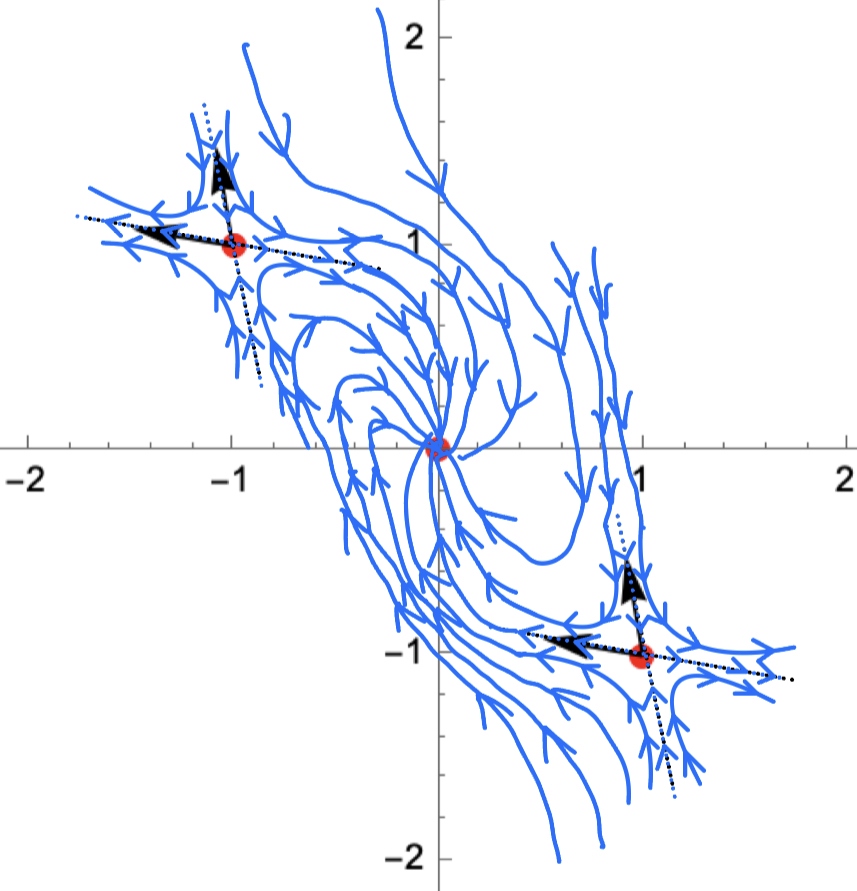
\includegraphics[width=.5\textwidth]{P1.jpg}
        \caption{Phase portrait for (P1). The equilibria are indicated with red points, and eigenvectors of the linearized system indicated with black arrows. The flow is indicated with the blue curves and arrows.}
    \end{figure}
    
    \item 
    \begin{align*}
        \dot{x}_1 &= x_1 + x_1 x_2 \\
        \dot{x}_2 &= -x_2 + x_2^2 + x_1 x_2 - x_1^3
    \end{align*}

    Equilibria are given by the system 
    \begin{align*}
        x_1 + x_1 x_2 &= 0\\
        -x_2 + x_2^2 + x_1 x_2 - x_1^3 &= 0
    \end{align*}
    The first of these gives $x_1 = 0$ or $x_2 = -1$. 
    For $x_1 = 0$ the second equation reduces to 
    $$ -x_2 + x_2^2 = 0$$
    which gives $x_2 = 0, 1$. 
    The case $x_2 = -1$ gives the equation 
    $$ 0 = 2 - x_1 - x_1^3 = (1-x_1)(x_1^2 + x_1 + 2)$$
    which gives $x_1 = 1$. The three equilibria are 
    $$ \textbf{x}_1 = ( 0,0), \hspace{.5cm} \textbf{x}_2 = ( 0,1), \text{ and } \textbf{x}_3 = (1,-1).$$
    
    $$
    Df(x_1,x_2) = \left(\begin{array}{cc}
     x_2+1 & x_1 \\
     x_2-3 x_1^2 & x_1+2 x_2-1 \\
    \end{array} \right)
    $$
    $$
    Df(\textbf{x}_1) = \left(\begin{array}{cc}
        1 & 0 \\
        0 & -1 \\
    \end{array}\right), \hspace{.5cm} 
    Df(\textbf{x}_2) = \left(\begin{array}{cc}
        2 & 0 \\
        1 & 1 \\
\end{array}\right),\hspace{.5cm} Df(\textbf{x}_3) = \left(\begin{array}{cc}
        0 & 1 \\
        -4 & -2 \\
\end{array}\right)$$
 
 $Df(\textbf{x}_1)$ has eigenvalues $\lambda = -1,1$ $\Rightarrow$ $\textbf{x}_1$ is a saddle point. $Df(\textbf{x}_2)$ has eigenvalues $\lambda = 1,2$ $\Rightarrow$ $\textbf{x}_2$ is an unstable node. $Df(\textbf{x}_3)$ has eigenvalues $\lambda = -1 \pm i \sqrt{3}$ $\Rightarrow$ $\textbf{x}_3$ is stable focus. 
\begin{figure}
        \centering
        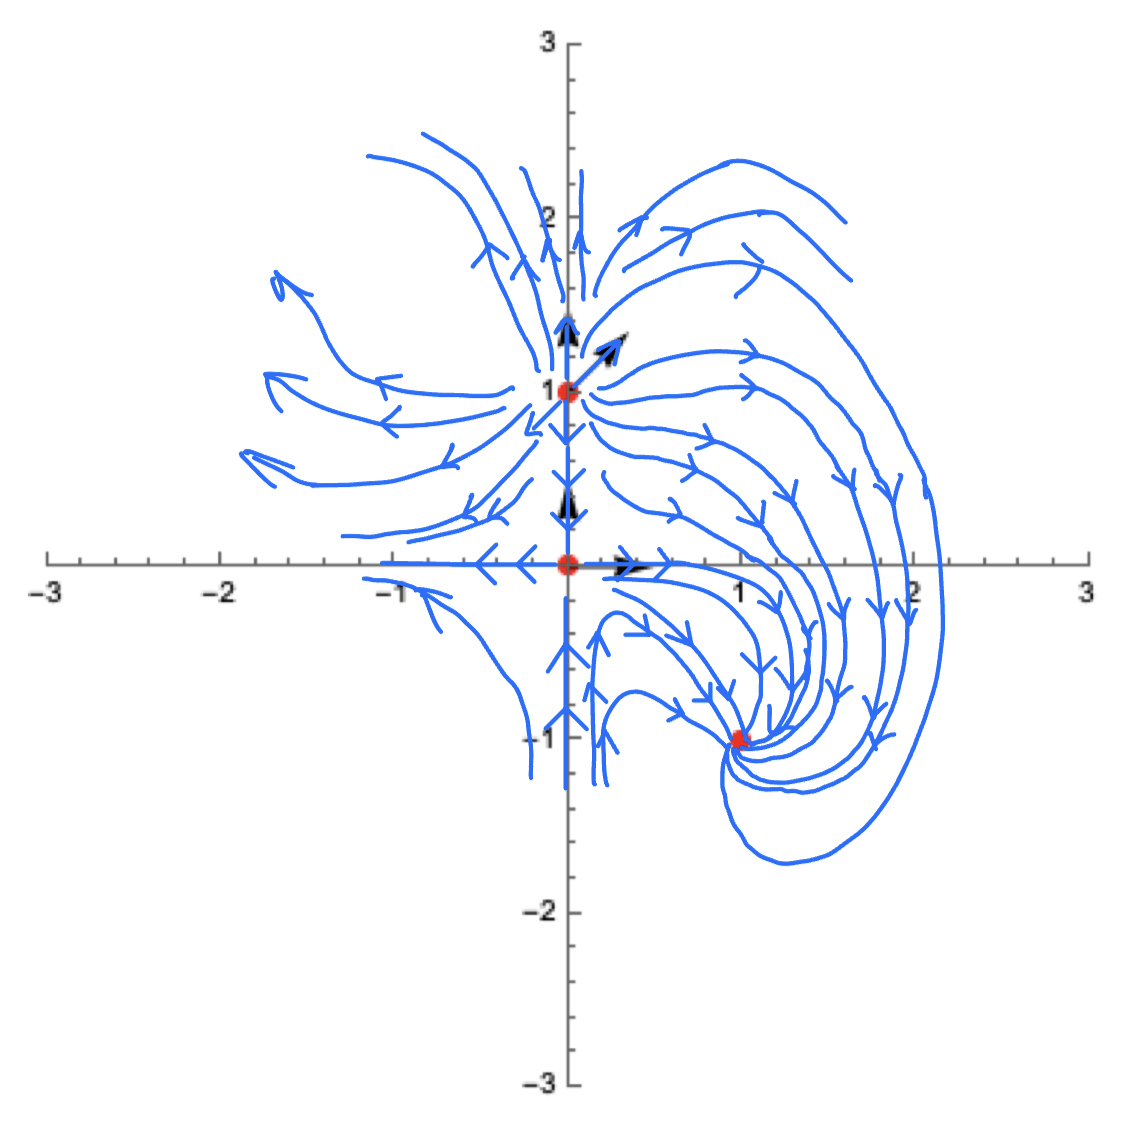
\includegraphics[width=.5\textwidth]{P2.jpeg}
        \caption{Phase portrait for (P1). The equilibria are indicated with red points, and eigenvectors of the linearized system indicated with black arrows. The flow is indicated with the blue curves and arrows.}
\end{figure}

\end{enumerate}
\end{solution}

\newpage
\begin{problem}
\begin{enumerate}[label=(P\arabic*)]
    \item Using $x_1 = \sigma$ and $x_2 = v$ as the state variables, find the state-space equation model of the system. 
    \item Let $v_d$ be a positive constant. Find all equilibrium points and determine the type of each point. 
    \item Discuss the qualitative behavior of the system for the given numerical values. 
\end{enumerate}
\end{problem}
\begin{solution}\
\begin{enumerate}[label=(P\arabic*)]
    \item The state space variables are 
    \begin{align*}
        x_1 &= \sigma \\
        x_2 &= v
    \end{align*}
    giving 
    \begin{align*}
        \dot{x}_1 &= v_d - x_2\\
        \dot{x}_2 &= \frac{1}{m}\left( K_I x_1 + K_p (v_d - x_2) -K_c \sgn(x_2) - K_f x_2 - K_a x_2^2\right)
    \end{align*}
    \item $v_d > 0$, $\dot{x}_1 = \dot{x}_2 = 0$ $\Rightarrow$
    \begin{align*}
        0 &= v_d - x_2 \Rightarrow x_2 = v_d\\
        0 &= \frac{1}{m}\left( K_I x_1 + K_p (v_d - x_2) -K_c \sgn(x_2) - K_f x_2 - K_a x_2^2\right)\\
        \Rightarrow 0 &= \frac{1}{m}\left( K_I x_1 - K_c - K_f v_d - K_a v_d^2\right)\\
        \Rightarrow x_1 &= \frac{1}{K_1}\left(K_c + K_f v_d + K_a v_d^2\right)
    \end{align*}
    $$ Df(\frac{1}{K_1}\left(K_c + K_f v_d + K_a v_d^2\right), v_d) = \begin{pmatrix} 0 & -1 \\ \frac{K_I}{m} & \frac{ -K_p - K_f - 2 K_a v_d}{m} \end{pmatrix}$$
    $Df$ has eigenvalues $ \lambda = \frac{-(K_f+K_p+2K_a v_d) \pm \sqrt{(K_f + K_p + 2 K_a v_d)^2 - 4 K_I m}}{2m}$
    When $K_p$ and $K_I$ are chosen to ensure $(K_f + K_p + 2 K_a v_d)^2 - 4 K_I m \geq 0$, the equilibrium is a stable node, and when $(K_f + K_p + 2 K_a v_d)^2 - 4 K_I m < 0$ the equilibrium is a stable focus. If $0 < (K_f + K_p + 2 K_a v_d) < 1$, then the equilibrium can be a sadle point for some choices of $K_I$. 
    \item The numerical values give $(x_1,x_2) = (72.333,30)$, and $ \lambda = -0.3461, -0.0289$. This makes the equilibrium a stable node.
\end{enumerate}
\end{solution}

\newpage
\begin{problem}
For each of the following systems, find and classify bifurcations that occur as $\mu$ varies. 
\begin{enumerate}[label=(P\arabic*)]
    \item $\dot{x}_1 = x_2$ and $\dot{x}_2 = \mu(x_1 + x_2) - x_2 - x_1^3 - 3 x_1^2 x_2$. 
    \item $\dot{x}_1 = x_2$ and $\dot{x}_2 = \mu - x_2 - x_1^2 - 2x_1 x_2$. 
\end{enumerate}
\end{problem}
\begin{solution}
	\begin{enumerate}[label=(P\arabic*)]
		\item $ x_2= 0$ and $\dot{x}_2 = \mu(x_1) - x_1^3 = 0$. This gives, 
			$x_1 = 0,\pm \sqrt{\mu}$. 
			$$
				Df(x_1,x_2) = 
				\begin{pmatrix} 
					0 & 1 \\ 
					\mu-3 x_1^2 - 6 x_1 x_2 & \mu - 1 -3 x_1^2
				\end{pmatrix}
			$$ 
			has eigenvalues 
		$$ 
			\lambda = \frac{1}{2} \left(\mu -3 x_1^2\pm \sqrt{\mu ^2+2 \mu +9 x_1^4-6 \mu  x_1^2-6 x_1^2-24 x_1 x_2+1}-1\right)
		$$
		
		When $x_1 = 0$, 
		$$
			\lambda = \frac{1}{2} \left(\mu \pm|\mu +1|-1\right).
		$$ 
		For $\mu < 0$, $\lambda$ are both negative and the equilibrium is a
		stable node. For $\mu > 0 $ one eigenvalue is negative and one is
		positive, so the equilibrium is a saddle point.
		
		When $x_1 = \pm \sqrt{\mu}$, $\lambda = -\mu \pm \frac{1}{2} |2 \mu
		-1|-\frac{1}{2}$. For $\mu < 0$, there is no equilibrium because
		$\sqrt{\mu}$ is imaginary. For $\mu > 0$, both eigenvalues are negative,
		and the equilibrium is a stable node. 
		
		This is a supercritical pitchfork bifurcation. 
		
		\begin{figure}[h]
			\centering
			\begin{tabular}{c c}
				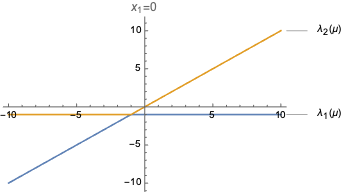
\includegraphics[width=.5\textwidth]{x10.png} & 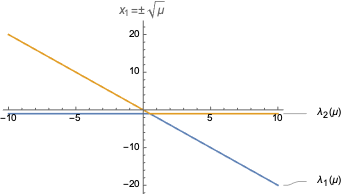
\includegraphics[width=.5\textwidth]{x1pm.png}
			\end{tabular}
			\caption{Plots of eigenvalues against $\mu$}
		\end{figure}
		\item $x_2 =0$ and $\dot{x}_2 = \mu - x_1^2 =0 $. This gives, $x_1 = \pm \sqrt{\mu}$. 
		$$
			Df(x_1,x_2) = 
			\begin{pmatrix} 
				0 & 1 \\ 
				-2 x_1 - 2 x_2 & -1 -2 x_1
			\end{pmatrix}
		$$
		$$
			Df(\pm\sqrt{\mu},0) = 
			\begin{pmatrix}
				0 & 1 \\
				\mp 2 \sqrt{\mu} & -1 \mp 2\sqrt{\mu}
			\end{pmatrix}
		$$
		has eigenvalues 
		\begin{align*} 
			\lambda_1 &= \frac{1}{2} \left(\left(-1\mp 2 \sqrt{\mu }\right)-\sqrt{\left(-1\mp 2 \sqrt{\mu }\right)^2+4 \sqrt{\mu } (\mp 2)}\right)\\
			\lambda_2 &= \frac{1}{2} \left(\left(-1\mp 2 \sqrt{\mu }\right)+\sqrt{\left(-1\mp 2 \sqrt{\mu }\right)^2+4 \sqrt{\mu } (\mp 2)}\right)
		\end{align*}
		
		For $x_1 = -\sqrt{\mu}$ this simplifies to 
		\begin{align*}
			\lambda_1 &= -1 \\
			\lambda_2 &= 2 \sqrt{\mu}
		\end{align*}
		
		For $x_1 = \sqrt{\mu}$
		this simplifies to 
		\begin{align*}
			\lambda_1 &= -1 \\
			\lambda_2 &= -2 \sqrt{\mu}
		\end{align*}
		\begin{figure}[h]
			\centering
			\begin{tabular}{c c}
				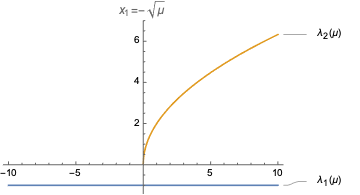
\includegraphics[width=.5\textwidth]{x21.png} & 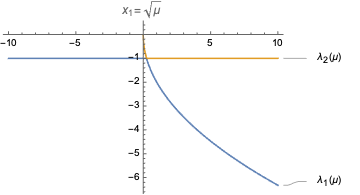
\includegraphics[width=.5\textwidth]{x22.png}
			\end{tabular}
			\caption{Plots of eigenvalues against $\mu$}
		\end{figure}
		
		For $\mu<0$, no equilibrium exists because $\sqrt{\mu}$ is imaginary.
		For $\mu>0$, $Df(x_1,x_2)$ has real eigenvalues with opposite sign at
		$x_1 = -\sqrt{\mu}$, and real negative eigenvalues at $x_1 = \sqrt{\mu}$.
		So for $\mu>0$, $x_1 = -\sqrt{\mu}$ is a saddle point and $x_1 = \sqrt{\mu}$
		is a stable node. This is a saddle-node bifurcation.
	\end{enumerate}
\end{solution}
\end{document}
